\documentclass{beamer}

\usepackage{lipsum}
\usepackage[utf8]{inputenc}
\usepackage[ngerman,english]{babel}
\usepackage{amsmath}
\usepackage{amsthm}
\usepackage{graphicx}
\usepackage{caption}
\usepackage{lmodern}
\usepackage{float}
\usepackage{sidecap}
\usepackage{pgfplots}
\usepackage{pgfplotstable}
\usepackage{tabularcalc}
\usepackage{todonotes}
\usepackage{hyperref}
\usepackage{minted}
\usepackage{siunitx}
\usepackage{subfig}
\usepackage[customcolors]{hf-tikz}
\usepackage{booktabs}
\graphicspath{{graphs/}}
\pgfplotsset{compat=1.12}

% Due to bug in subfig
\makeatletter
\let\@@magyar@captionfix\relax
\makeatother

\title[Privacy Implications of Exposing Git Metadata]
{Privacy Implications of Exposing Git Meta Data}
\author[Beer]{Arne Beer \\ \footnotesize Matriculation number: 6489196}
\institute[University of Hamburg]{
    Department of Computer Science\\
    University of Hamburg
}
\subject{Computer Science}

\usetheme{Szeged}
\usecolortheme{seagull}

\begin{document}
\frame{\titlepage}
\begin{frame}
    \frametitle{Table of Contents}
    \footnotesize
    \tableofcontents
\end{frame}

\section{Introduction}

\subsection{Topic}
\begin{frame}
    \frametitle{Topic}
    \begin{block}{Main topic of the thesis}
        Can Git metadata be maliciously used?
    \end{block}
\end{frame}

\subsection{Motivation}
\begin{frame}
    \frametitle{Motivation}
    \begin{itemize}
        \item Used in nearly every project
        \pause{}
        \item No obvious leak of personal information
        \pause{}
        \item Possible workplace/contributor surveillance
    \end{itemize}
\end{frame}

\subsection{Leading Question and Goals}
\begin{frame}
    \frametitle{Leading Question and Goals}
    \begin{itemize}
        \item Feasibility of scanning repositories on different scales
        \item Possible extraction of interesting information
        \item Possible attack vectors
    \end{itemize}
\end{frame}

\section{Aggregation}

\subsection{Data Source}
\begin{frame}
    \frametitle{Why Github?}
    \begin{itemize}
        \item Largest accumulation of open-source Git repositories
        \pause{}
        \item Great API
        \pause{}
        \item Allows exploration
    \end{itemize}
\end{frame}

\begin{frame}
    \frametitle{Exploration}
    \begin{itemize}
        \item Repository ownership
        \item Stars
        \item Following
    \end{itemize}
\end{frame}


\begin{frame}
    \frametitle{Gitalizer}
    \begin{itemize}
        \item Crawls Github
        \item Starts at user or company
        \item Highly optimized
    \end{itemize}
\end{frame}

\section{Attack Models}
\subsection{Attack Models}
\begin{frame}
    \frametitle{The Three Attack Models}
    \begin{itemize}
        \item Employer
        \pause{}
        \item Individual
        \pause{}
        \item Industrial Spy
    \end{itemize}
\end{frame}

\subsection{Attacks}
\begin{frame}
    \frametitle{Three Chosen Attacks}
    \begin{itemize}
        \item Holiday and Sick Leave Detection
        \pause{}
        \item Sleep Rhythm and Working Hours
        \pause{}
        \item Geographic Location
    \end{itemize}
\end{frame}

\section{Research}
\subsection{Holiday and Sick Leave}
\begin{frame}
    \frametitle{Holiday and Sick Leave: Goals}
    \begin{itemize}
        \item Automatic detection
        \pause{}
        \item Accurate detection
    \end{itemize}
\end{frame}

\begin{frame}
    \frametitle{Example}
    \begin{figure}[H]
        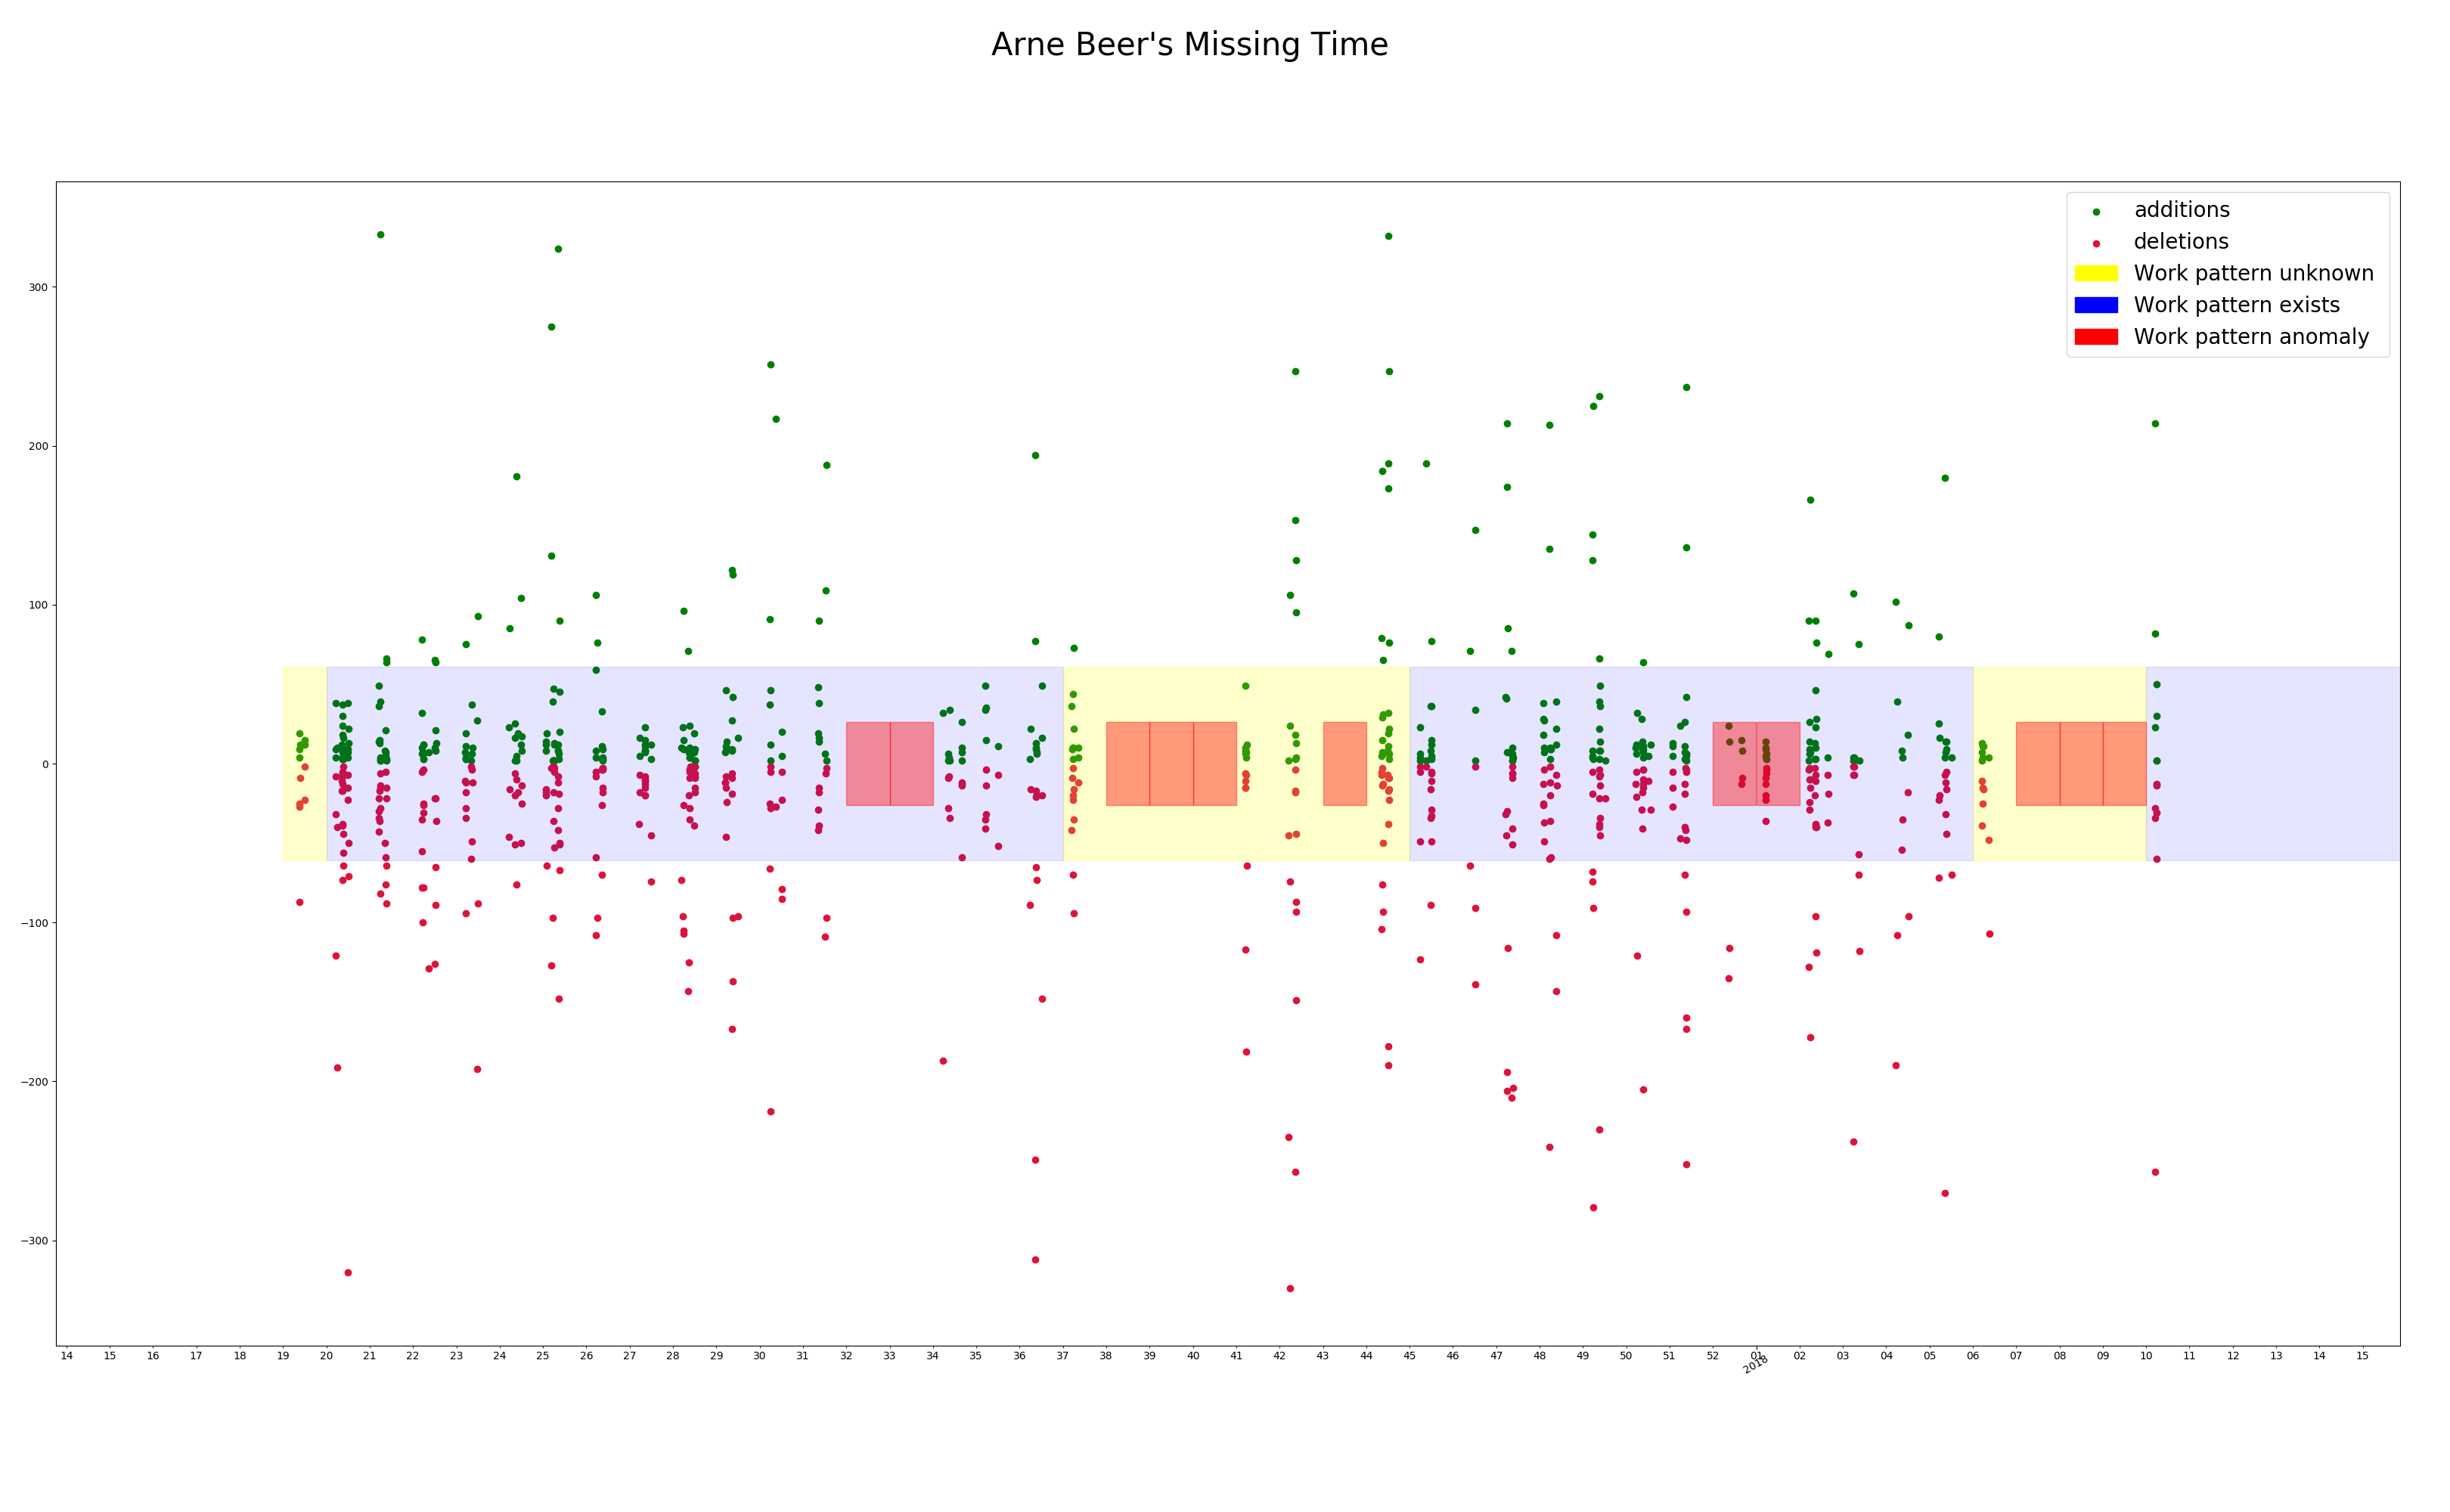
\includegraphics[scale=0.115]{analysis/work-time-analysis}
        \centering
        \caption{Holiday and Sick leave visualization}
    \end{figure}
\end{frame}

\begin{frame}
    \frametitle{Results}
    \begin{itemize}
        \item Tested in a small company
        \pause{}
        \item Quite accurate
        \pause{}
        \item Needs interpretation
    \end{itemize}
\end{frame}

\subsection{Sleep Rhythm and Working Hours}
\begin{frame}
    \frametitle{Sleep Rhythm and Working Hours: Goals}
    \begin{itemize}
        \item Detection
        \pause{}
        \item Good visualization
        \pause{}
        \item Further implications of rhythm
    \end{itemize}
\end{frame}

\begin{frame}
    \frametitle{Example}
    \begin{figure}[H]
        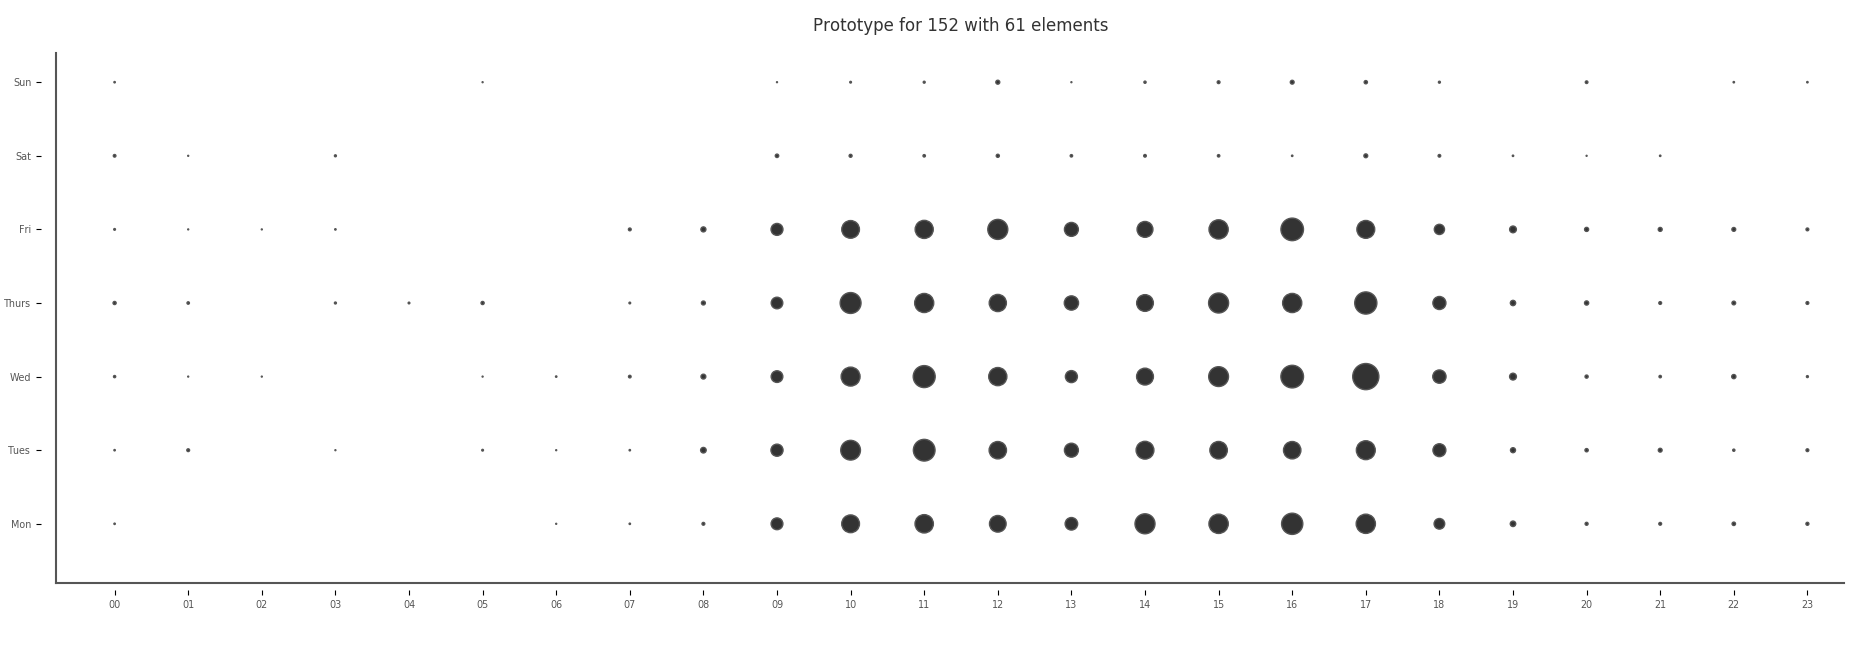
\includegraphics[scale=0.22]{analysis-affinity/152}
        \centering
        \caption{Regular working hour cluster}
    \end{figure}
\end{frame}

\begin{frame}
    \frametitle{Example}
    \begin{figure}[H]
        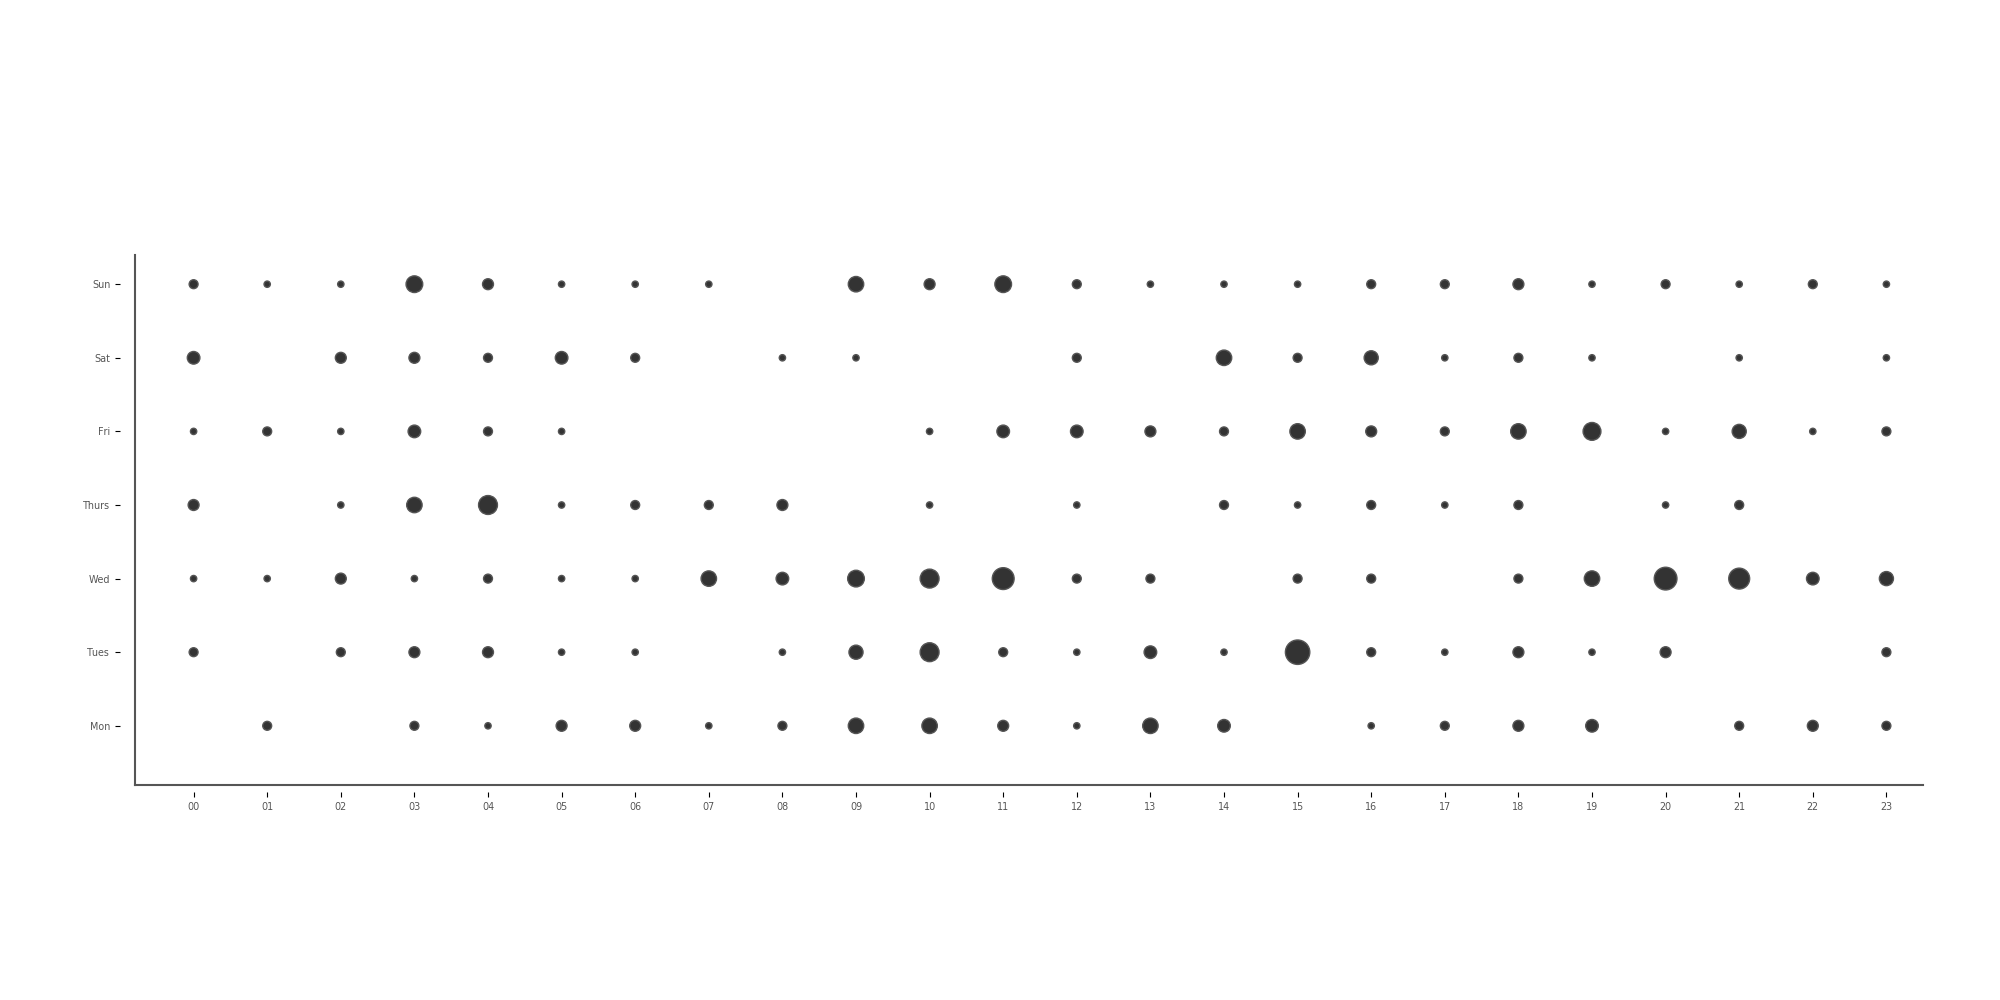
\includegraphics[scale=0.22]{analysis/random-punchcard}
        \centering
        \caption{Person without a sleep rhythm}
    \end{figure}
\end{frame}


\begin{frame}
    \frametitle{Results}
    \begin{itemize}
        \item Shows general tendency
        \pause{}
        \item Unsuitable for direct personal mapping
        \pause{}
        \item Allows to guess further information
    \end{itemize}
\end{frame}


\subsection{Geographic Location}
\begin{frame}
    \frametitle{Geographic Location: Goals}
    \begin{itemize}
        \item Detect holiday destinations
        \pause{}
        \item Detect home country
        \pause{}
        \item Detect time periods
    \end{itemize}
\end{frame}

\begin{frame}
    \frametitle{Methodology}
    \begin{itemize}
        \item Periodically check commits
        \pause{}
        \item Daylight Savings Time
    \end{itemize}
\end{frame}

\begin{frame}
    \frametitle{Example}
    \begin{figure}[H]
        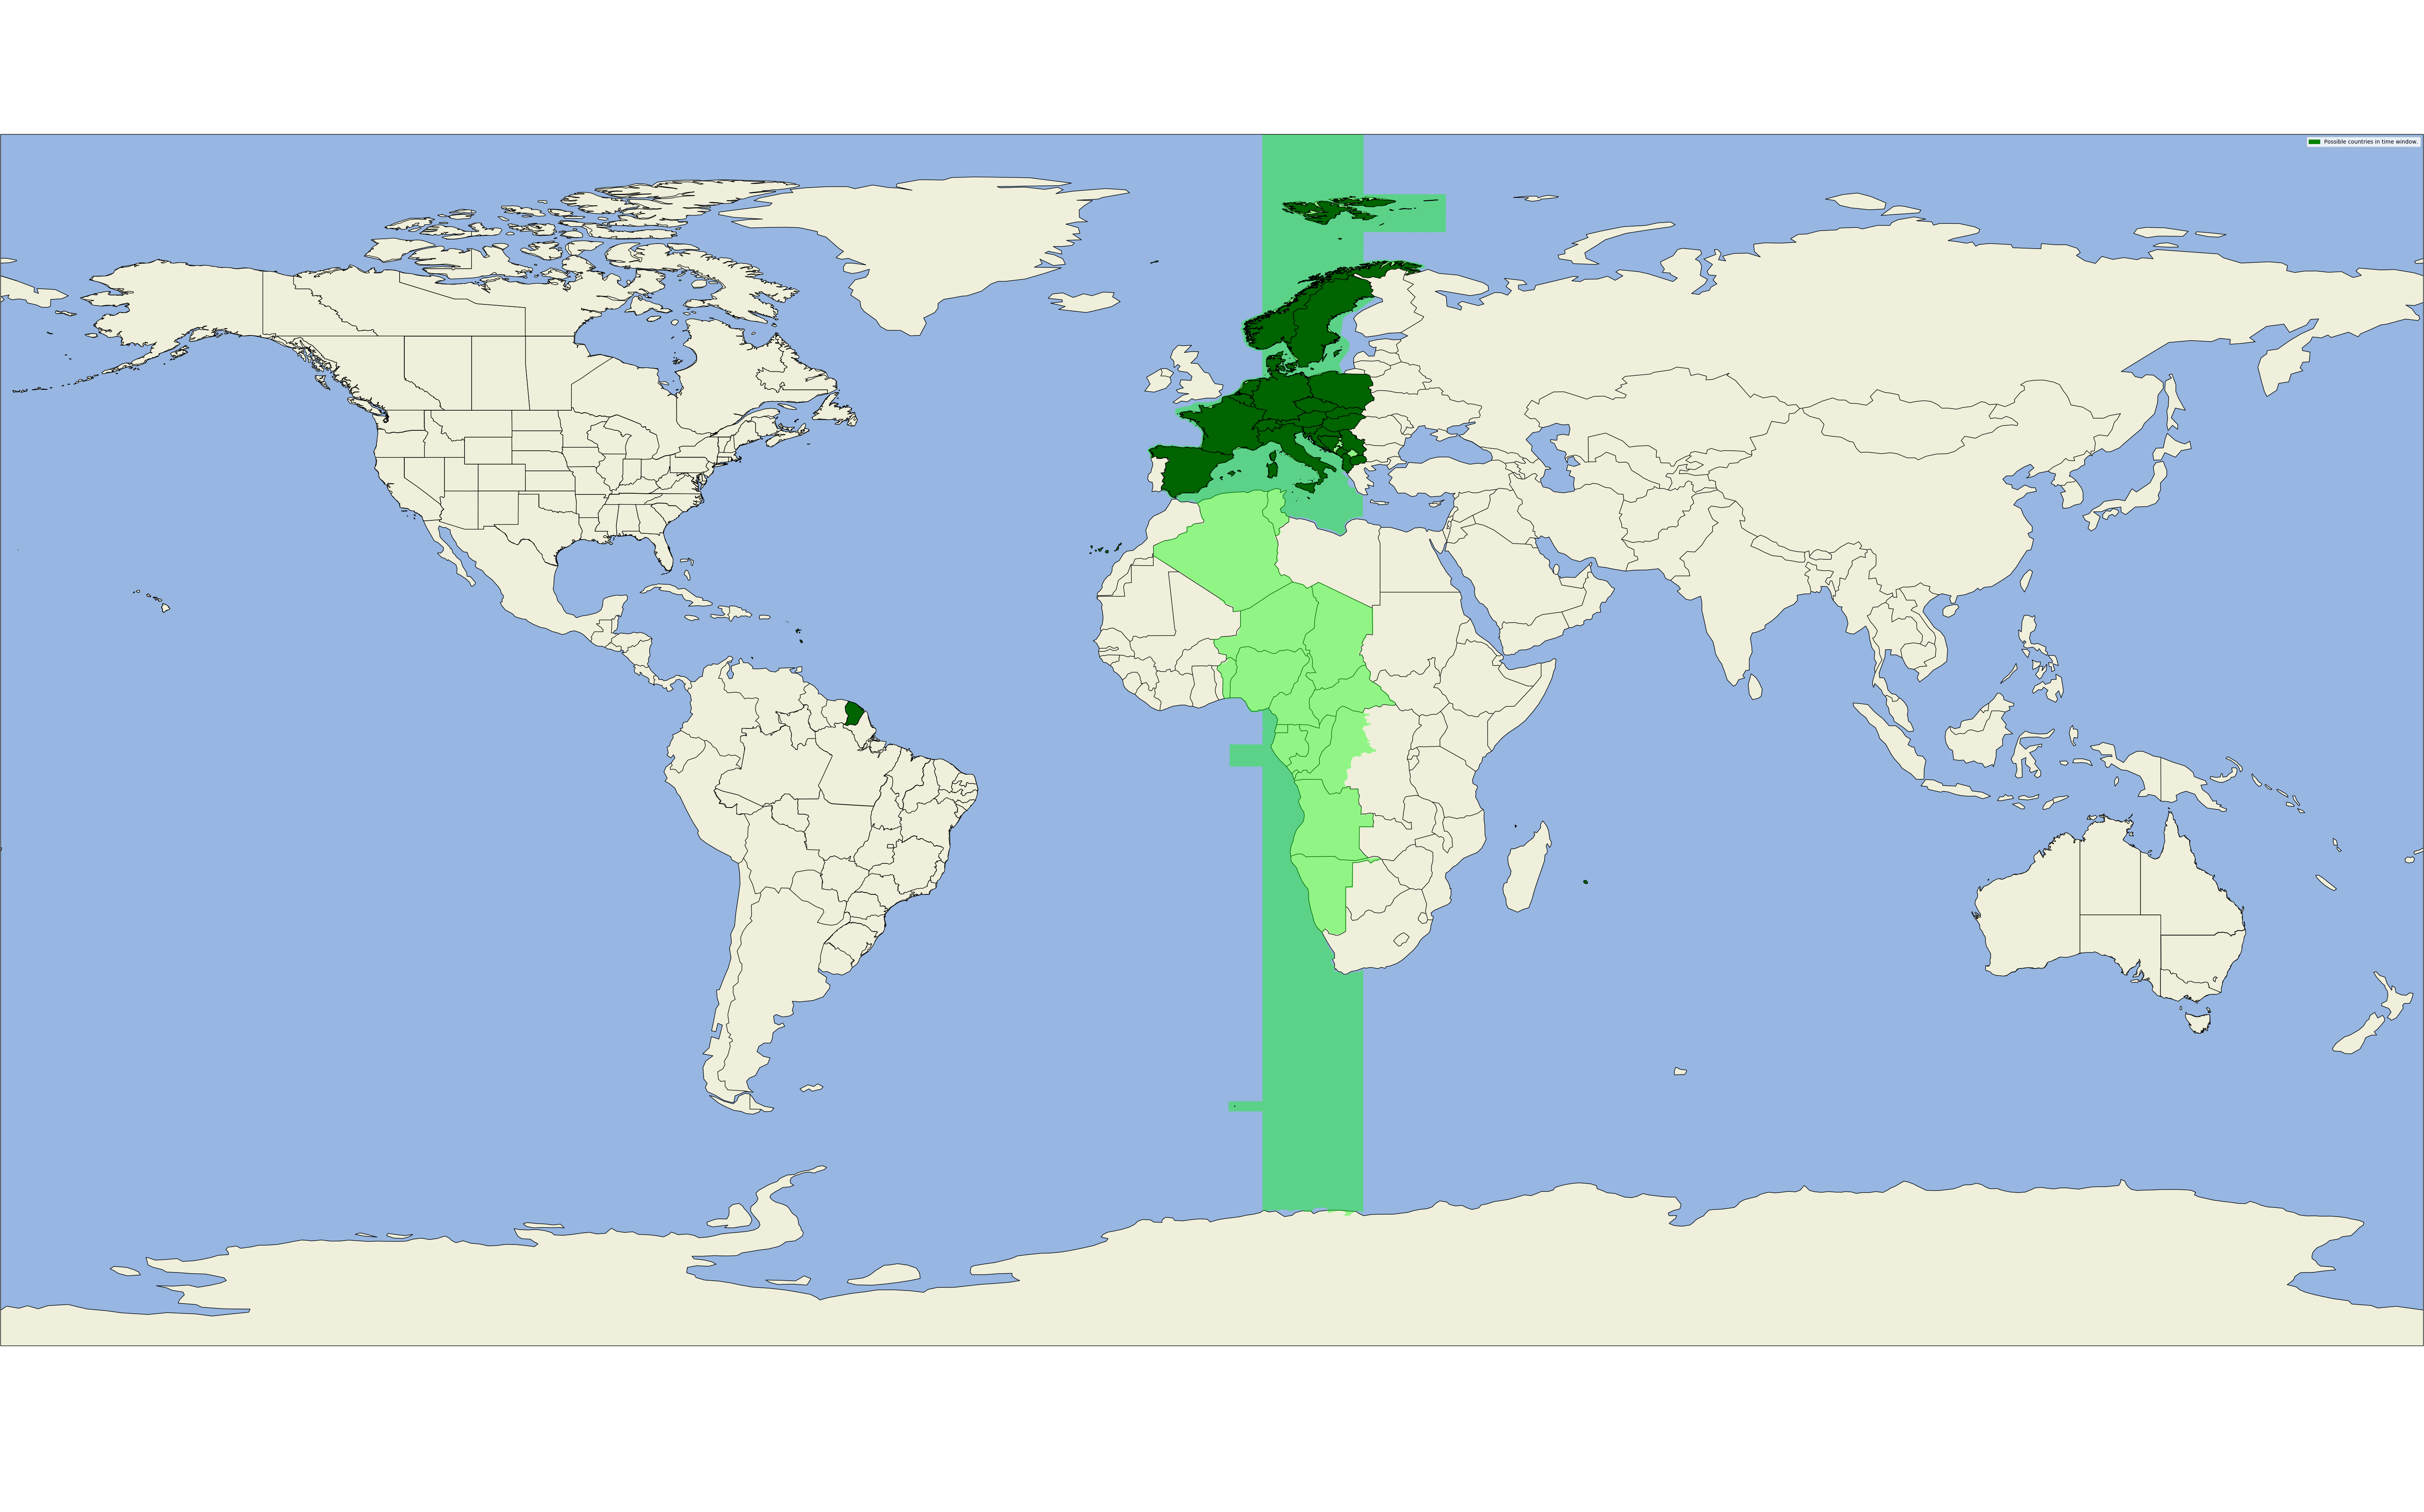
\includegraphics[scale=0.06]{analysis/author-home-location}
        \centering
        \caption{Home location analysis}
    \end{figure}
\end{frame}

\begin{frame}
    \frametitle{Results}
    \begin{itemize}
        \item Good detection of home country
        \pause{}
        \item Holiday not checked
        \pause{}
        \item Needs better libraries
    \end{itemize}
\end{frame}

\section{Conclusion and Outlook}
\subsection{Conclusion}
\begin{frame}
    \frametitle{Conclusion}
    \begin{itemize}
        \item Recall the goal: Is it possible to extract personal information
        \pause{}
        \item Scanning on small to middle scale
    \end{itemize}
\end{frame}

\subsection{Outlook}
\begin{frame}
    \frametitle{Outlook}
    \begin{itemize}
        \item It can become a problem
        \pause{}
        \item Many more complex and promising attack vectors
        \pause{}
        \item Methodologies to obfuscate data
    \end{itemize}
\end{frame}


\begin{frame}
    \frametitle{Fin}
    Thank you for your attention.
\end{frame}
\end{document}
